%!TEX TS-program = lualatex
\documentclass[
	ngerman,
	twoside,
	pdfa=false,
	ruledheaders=section,%Ebene bis zu der die Überschriften mit Linien abgetrennt werden, vgl. DEMO-TUDaPub
	class=report,% Basisdokumentenklasse. Wählt die Korrespondierende KOMA-Script Klasse
	thesis={type=Übung},% Dokumententyp Thesis, für Dissertationen siehe die Demo-Datei DEMO-TUDaPhd
	accentcolor=TUDa-9d,% Auswahl der Akzentfarbe
	custommargins=false,% Ränder werden mithilfe von typearea automatisch berechnet
	marginpar=false,% Kopfzeile und Fußzeile erstrecken sich nicht über die Randnotizspalte
	%BCOR=5mm,%Bindekorrektur, falls notwendig
	parskip=half-,%Absatzkennzeichnung durch Abstand vgl. KOMA-Sript
	fontsize=11pt,%Basisschriftgröße laut Corporate Design ist mit 9pt häufig zu klein
%	logofile=tuda_logo.pdf, %Falls die Logo Dateien nicht installiert sind
]{tudapub}

% Sprachanpassung
\usepackage[english, main=ngerman]{babel}
\usepackage[autostyle]{csquotes}
\usepackage{microtype}
\usepackage{listings}
\usepackage{array}

% Literaturverzeichnis
\usepackage{biblatex}
\addbibresource{literature.bib}

% Pakete-Mathematik & mehr
\usepackage{mathtools}
\usepackage{amsmath}
\usepackage{amsfonts}
\usepackage{subcaption}
\usepackage{color}

% neu cmds
\newcommand*\diff{\mathop{}\!\mathrm{d}}
\newcommand*\Diff[1]{\mathop{}\!\mathrm{d^#1}}


\begin{document}
	\title{Software Engineering Übung 07}
	\subtitle{Design Pattern}
	\author[J. Lippert \and M. Dierking]
	{Jonathan Lippert \and Magnus Dierking}
	%\reviewer{}
	%\department{ce}

	
	\submissiondate{\today}
	

	\maketitle
	\pagenumbering{gobble}


	% Kurzzusammenfassung
%	\include{chapters/zusammenfassung}

	% Inhaltsverzeichnis 
%	\tableofcontents
	\newpage
	\pagenumbering{arabic}
	\setcounter{page}{1}
	

%-------------------------------------------------------------------------------------------------
     \chapter{Aufgabe 1}

\lstset{language=Java,
	showspaces=false,
	showtabs=false,
	breaklines=true,
	showstringspaces=false,
	breakatwhitespace=true,
}


\definecolor{dkgreen}{rgb}{0,0.6,0}
\definecolor{gray}{rgb}{0.5,0.5,0.5}
\definecolor{mauve}{rgb}{0.58,0,0.82}

\lstset{	
	frame=tb,
	language=Java,
	aboveskip=3mm,
	belowskip=3mm,
	showstringspaces=false,
	columns=flexible,
	basicstyle={\small\ttfamily},
	numbers=none,
	numberstyle=\tiny\color{gray},
	keywordstyle=\color{blue},
	commentstyle=\color{dkgreen},
	stringstyle=\color{mauve},
	breaklines=true,
	breakatwhitespace=true,
	tabsize=3,
	backgroundcolor=\color{black!5},
	numbers=left, stepnumber=1, numberstyle = \tiny
	% set backgroundcolor
}

\section{a}
\begin{figure}[h!]
	\centering
	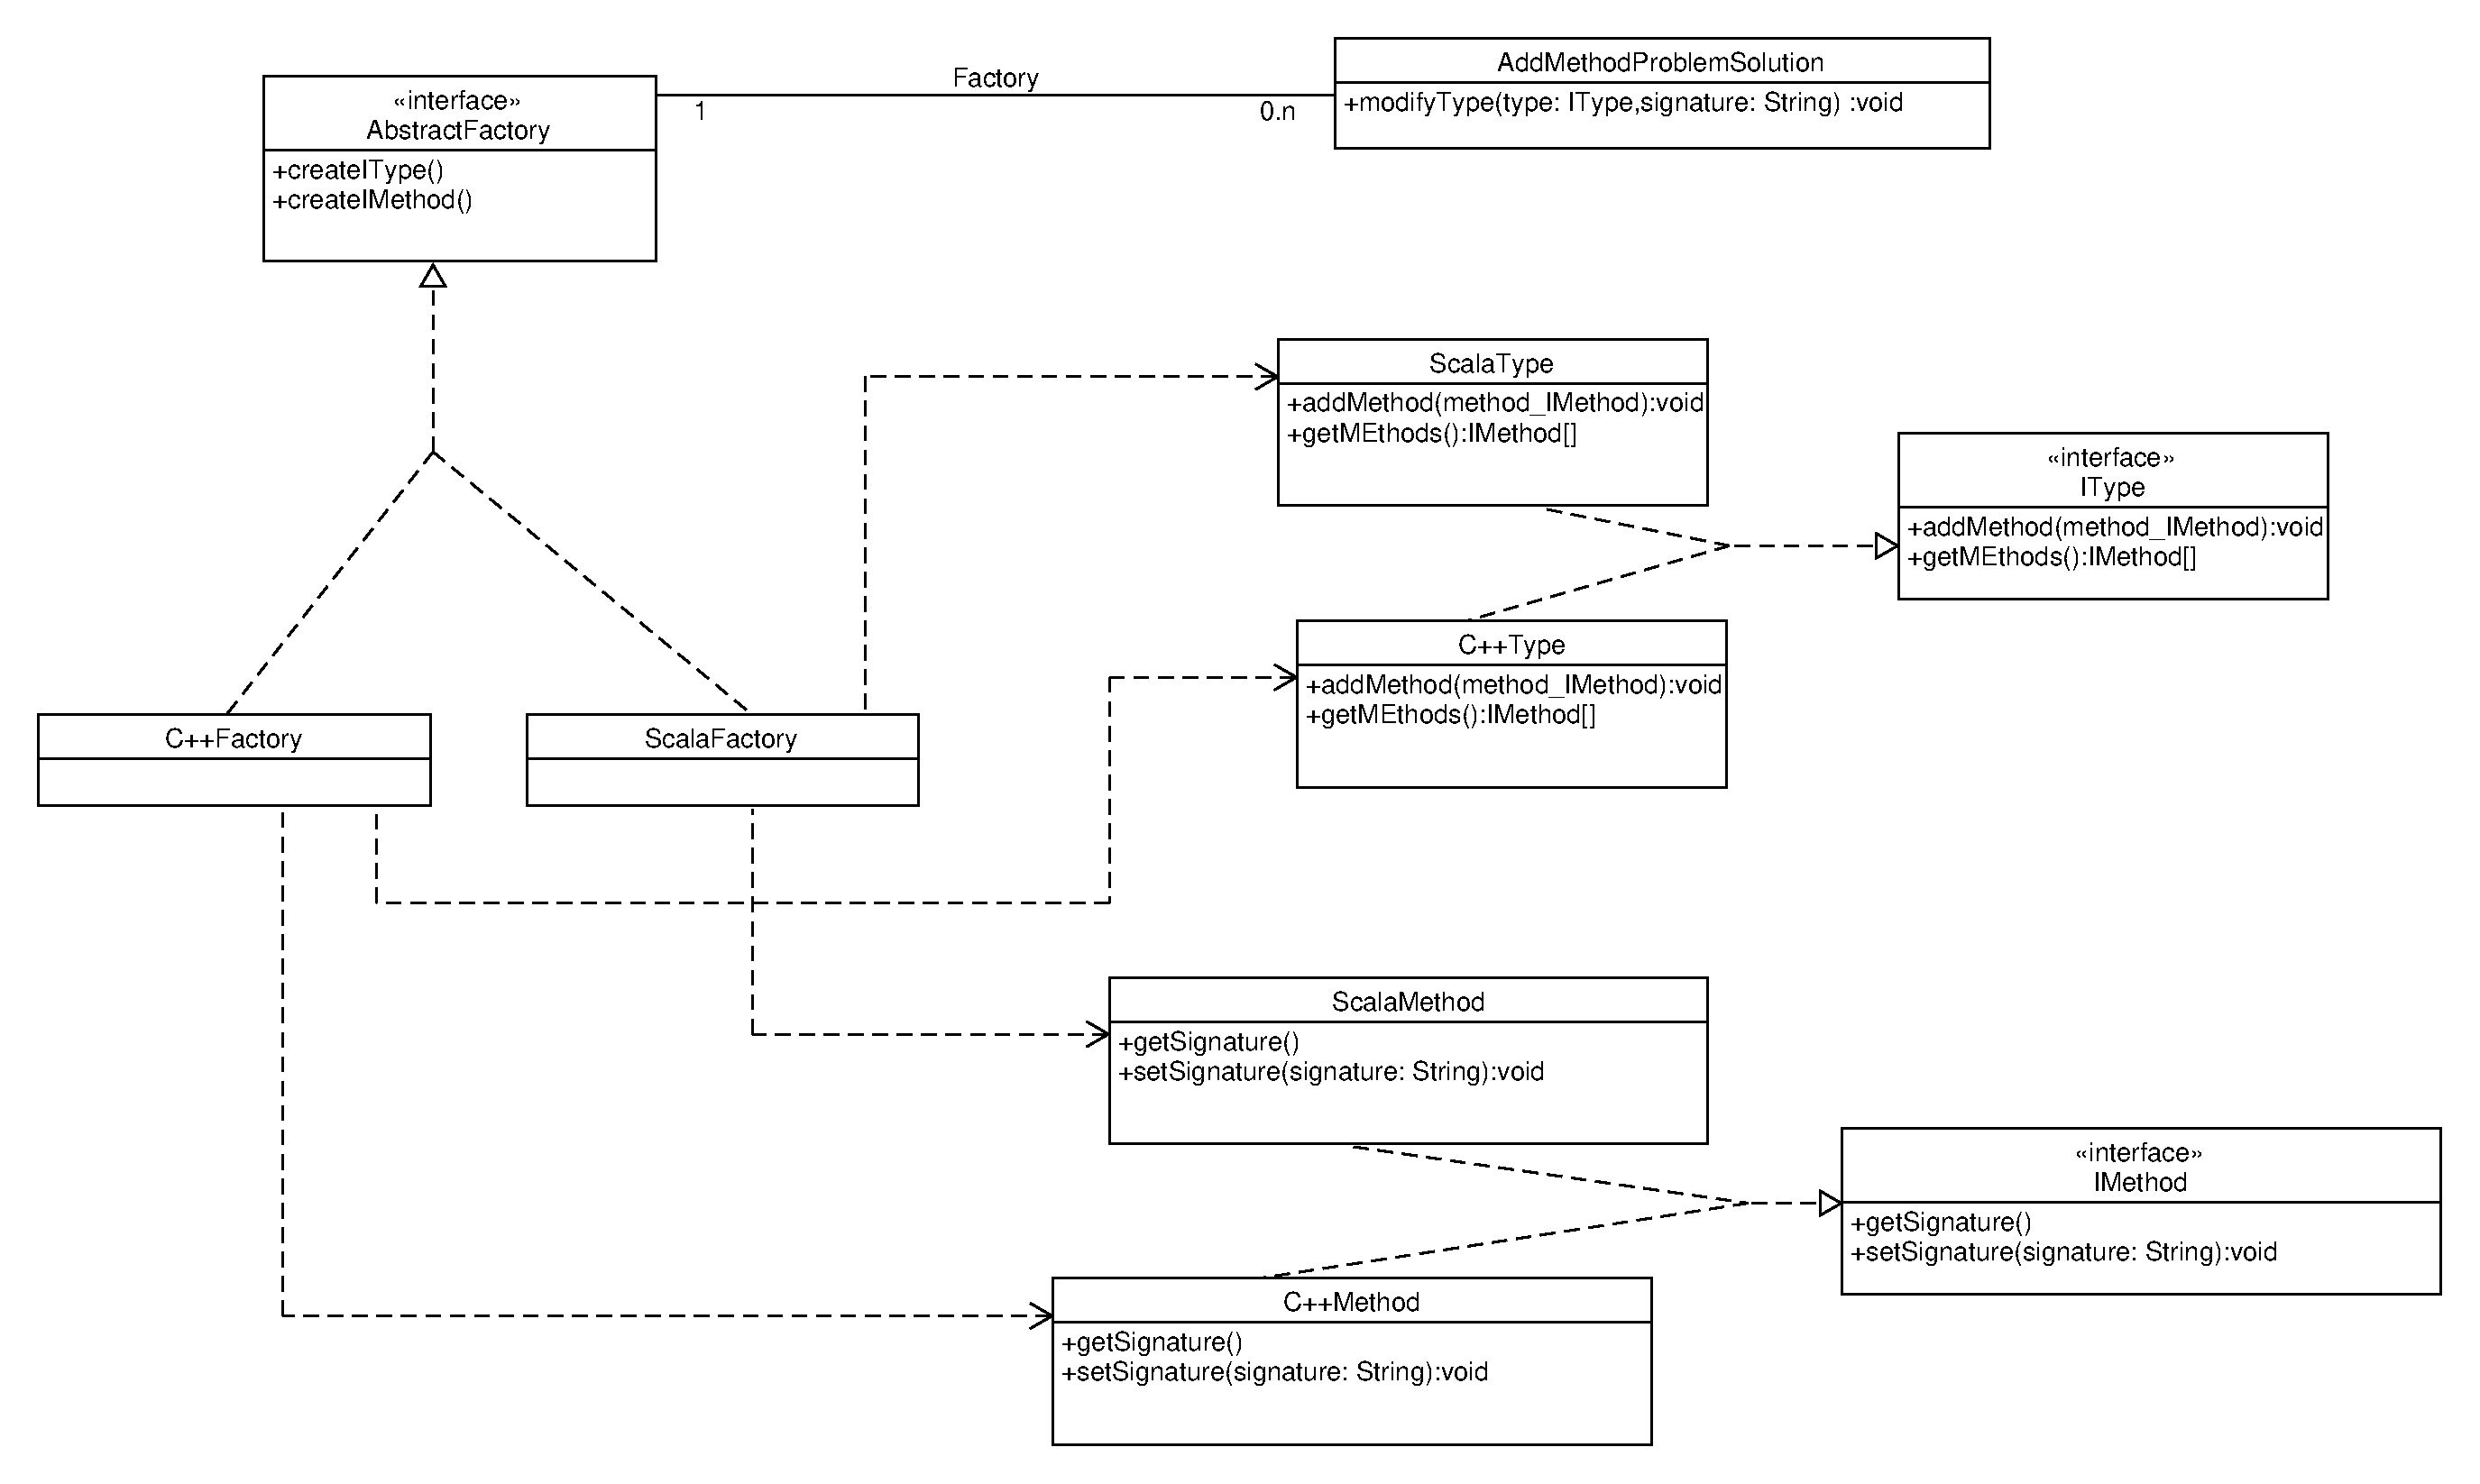
\includegraphics[width=0.8\textwidth, clip]{images/AbstractFactoryMyIDE_UML.pdf}
	\caption{UML Diagramm von MyIDE mit  AbstractFactory Pattern.}
	\label{fig:ULM}
\end{figure}
\section{b}


\begin{lstlisting}[ caption = {Aufgabe 1 b}]
	public ScalaMethod createIMethod(){  //retruntype evtl IMethod
		retrun new ScalaMethod();
	}
\end{lstlisting}


\section{c}
\begin{lstlisting}[caption = {Aufgabe 1 c}]
public void modifyType(IType type, String signature){
 	IMethod newMethod = factory.createIMethod();
 	newMethod.setSignature(signature);
	type.addMethod(newMethod);
}
\end{lstlisting}

\section{d}
Abstrakte Produkte:\\
IType, IMethod\\


Konkrete Implemntierung der abstrakten Fabrik:\\
ScalaFactory, C++Factory\\


Konkrete Implementierung der Produkte:\\
ScalaType, C++Type, ScalaMethod, C++Method\\


Methoden zum Erstellen von Produkten:\\
createIType, createIMethod\\


Abstrakte Fabrik:\\
AbstractFactory\\




%
%\begin{lstlisting}[	caption = {Klasse Book}]
%package org.library;
%
%
%public String getAuthor() { return author; }
%
%// implementiert interface LibraryItem
%@Override
%public String getCatalogDescription() {
%return title + " by " + author;  
%}
%}
%\end{lstlisting}



     %\chapter{Aufgabe 2}
\section{}
Die Klasse \texttt{Book} ist direkt abhängig von:
\begin{enumerate}
	\item Klasse \texttt{Client}
	\item Klasse \texttt{Date}
	\item Klasse \texttt{CSVExporter}
	\item Klasse \texttt{String}
	\item Klasse \texttt{IOException}
	\item Interface \texttt{LibraryItem}

\end{enumerate}

\section{}
Die Kopplung ist mit 6 für eine so allgemein gebräuchliche Klasse wie \texttt{Book} sehr hoch.
Änderungen in den all den anderen Klassen / Interfaces müssten in \texttt{Book} berücksichtigt werden. 
Ein Buch kann als Objekt jedoch auch abseits einer Bibliotheks-Implementation oft Anwendung finden, was eine Wiederverwendung sehr wahrscheinlich macht.
\\ 
Unter dem Aspekt des Responsibility-Driven Designs macht es zudem mehr Sinn, die nicht buch-spezifischen Funktionalitäten auszulagern.
Unserer Ansicht nach wären getrennte Klassen für das Exportieren, das Buch mit seinen String-Attributen und für die bibliotheks-spezifischen Dinge wie Verfügbarkeit etc. wünschenswerter.  

	
%-------------------------------------------------------------------------------------------------

	% Literaturverzeichnis
	\printbibliography % Erstellt die Bibliography
	
%	\include{chapters/anhang}
	

\end{document}